\documentclass[1p]{elsarticle_modified}
%\bibliographystyle{elsarticle-num}

%\usepackage[colorlinks]{hyperref}
%\usepackage{abbrmath_seonhwa} %\Abb, \Ascr, \Acal ,\Abf, \Afrak
\usepackage{amsfonts}
\usepackage{amssymb}
\usepackage{amsmath}
\usepackage{amsthm}
\usepackage{scalefnt}
\usepackage{amsbsy}
\usepackage{kotex}
\usepackage{caption}
\usepackage{subfig}
\usepackage{color}
\usepackage{graphicx}
\usepackage{xcolor} %% white, black, red, green, blue, cyan, magenta, yellow
\usepackage{float}
\usepackage{setspace}
\usepackage{hyperref}

\usepackage{tikz}
\usetikzlibrary{arrows}

\usepackage{multirow}
\usepackage{array} % fixed length table
\usepackage{hhline}

%%%%%%%%%%%%%%%%%%%%%
\makeatletter
\renewcommand*\env@matrix[1][\arraystretch]{%
	\edef\arraystretch{#1}%
	\hskip -\arraycolsep
	\let\@ifnextchar\new@ifnextchar
	\array{*\c@MaxMatrixCols c}}
\makeatother %https://tex.stackexchange.com/questions/14071/how-can-i-increase-the-line-spacing-in-a-matrix
%%%%%%%%%%%%%%%

\usepackage[normalem]{ulem}

\newcommand{\msout}[1]{\ifmmode\text{\sout{\ensuremath{#1}}}\else\sout{#1}\fi}
%SOURCE: \msout is \stkout macro in https://tex.stackexchange.com/questions/20609/strikeout-in-math-mode

\newcommand{\cancel}[1]{
	\ifmmode
	{\color{red}\msout{#1}}
	\else
	{\color{red}\sout{#1}}
	\fi
}

\newcommand{\add}[1]{
	{\color{blue}\uwave{#1}}
}

\newcommand{\replace}[2]{
	\ifmmode
	{\color{red}\msout{#1}}{\color{blue}\uwave{#2}}
	\else
	{\color{red}\sout{#1}}{\color{blue}\uwave{#2}}
	\fi
}

\newcommand{\Sol}{\mathcal{S}} %segment
\newcommand{\D}{D} %diagram
\newcommand{\A}{\mathcal{A}} %arc


%%%%%%%%%%%%%%%%%%%%%%%%%%%%%5 test

\def\sl{\operatorname{\textup{SL}}(2,\Cbb)}
\def\psl{\operatorname{\textup{PSL}}(2,\Cbb)}
\def\quan{\mkern 1mu \triangleright \mkern 1mu}

\theoremstyle{definition}
\newtheorem{thm}{Theorem}[section]
\newtheorem{prop}[thm]{Proposition}
\newtheorem{lem}[thm]{Lemma}
\newtheorem{ques}[thm]{Question}
\newtheorem{cor}[thm]{Corollary}
\newtheorem{defn}[thm]{Definition}
\newtheorem{exam}[thm]{Example}
\newtheorem{rmk}[thm]{Remark}
\newtheorem{alg}[thm]{Algorithm}

\newcommand{\I}{\sqrt{-1}}
\begin{document}

%\begin{frontmatter}
%
%\title{Boundary parabolic representations of knots up to 8 crossings}
%
%%% Group authors per affiliation:
%\author{Yunhi Cho} 
%\address{Department of Mathematics, University of Seoul, Seoul, Korea}
%\ead{yhcho@uos.ac.kr}
%
%
%\author{Seonhwa Kim} %\fnref{s_kim}}
%\address{Center for Geometry and Physics, Institute for Basic Science, Pohang, 37673, Korea}
%\ead{ryeona17@ibs.re.kr}
%
%\author{Hyuk Kim}
%\address{Department of Mathematical Sciences, Seoul National University, Seoul 08826, Korea}
%\ead{hyukkim@snu.ac.kr}
%
%\author{Seokbeom Yoon}
%\address{Department of Mathematical Sciences, Seoul National University, Seoul, 08826,  Korea}
%\ead{sbyoon15@snu.ac.kr}
%
%\begin{abstract}
%We find all boundary parabolic representation of knots up to 8 crossings.
%
%\end{abstract}
%\begin{keyword}
%    \MSC[2010] 57M25 
%\end{keyword}
%
%\end{frontmatter}

%\linenumbers
%\tableofcontents
%
\newcommand\colored[1]{\textcolor{white}{\rule[-0.35ex]{0.8em}{1.4ex}}\kern-0.8em\color{red} #1}%
%\newcommand\colored[1]{\textcolor{white}{ #1}\kern-2.17ex	\textcolor{white}{ #1}\kern-1.81ex	\textcolor{white}{ #1}\kern-2.15ex\color{red}#1	}

{\Large $\underline{11n_{17}~(K11n_{17})}$}

\setlength{\tabcolsep}{10pt}
\renewcommand{\arraystretch}{1.6}
\vspace{1cm}\begin{tabular}{m{100pt}>{\centering\arraybackslash}m{274pt}}
\multirow{5}{120pt}{
	\centering
	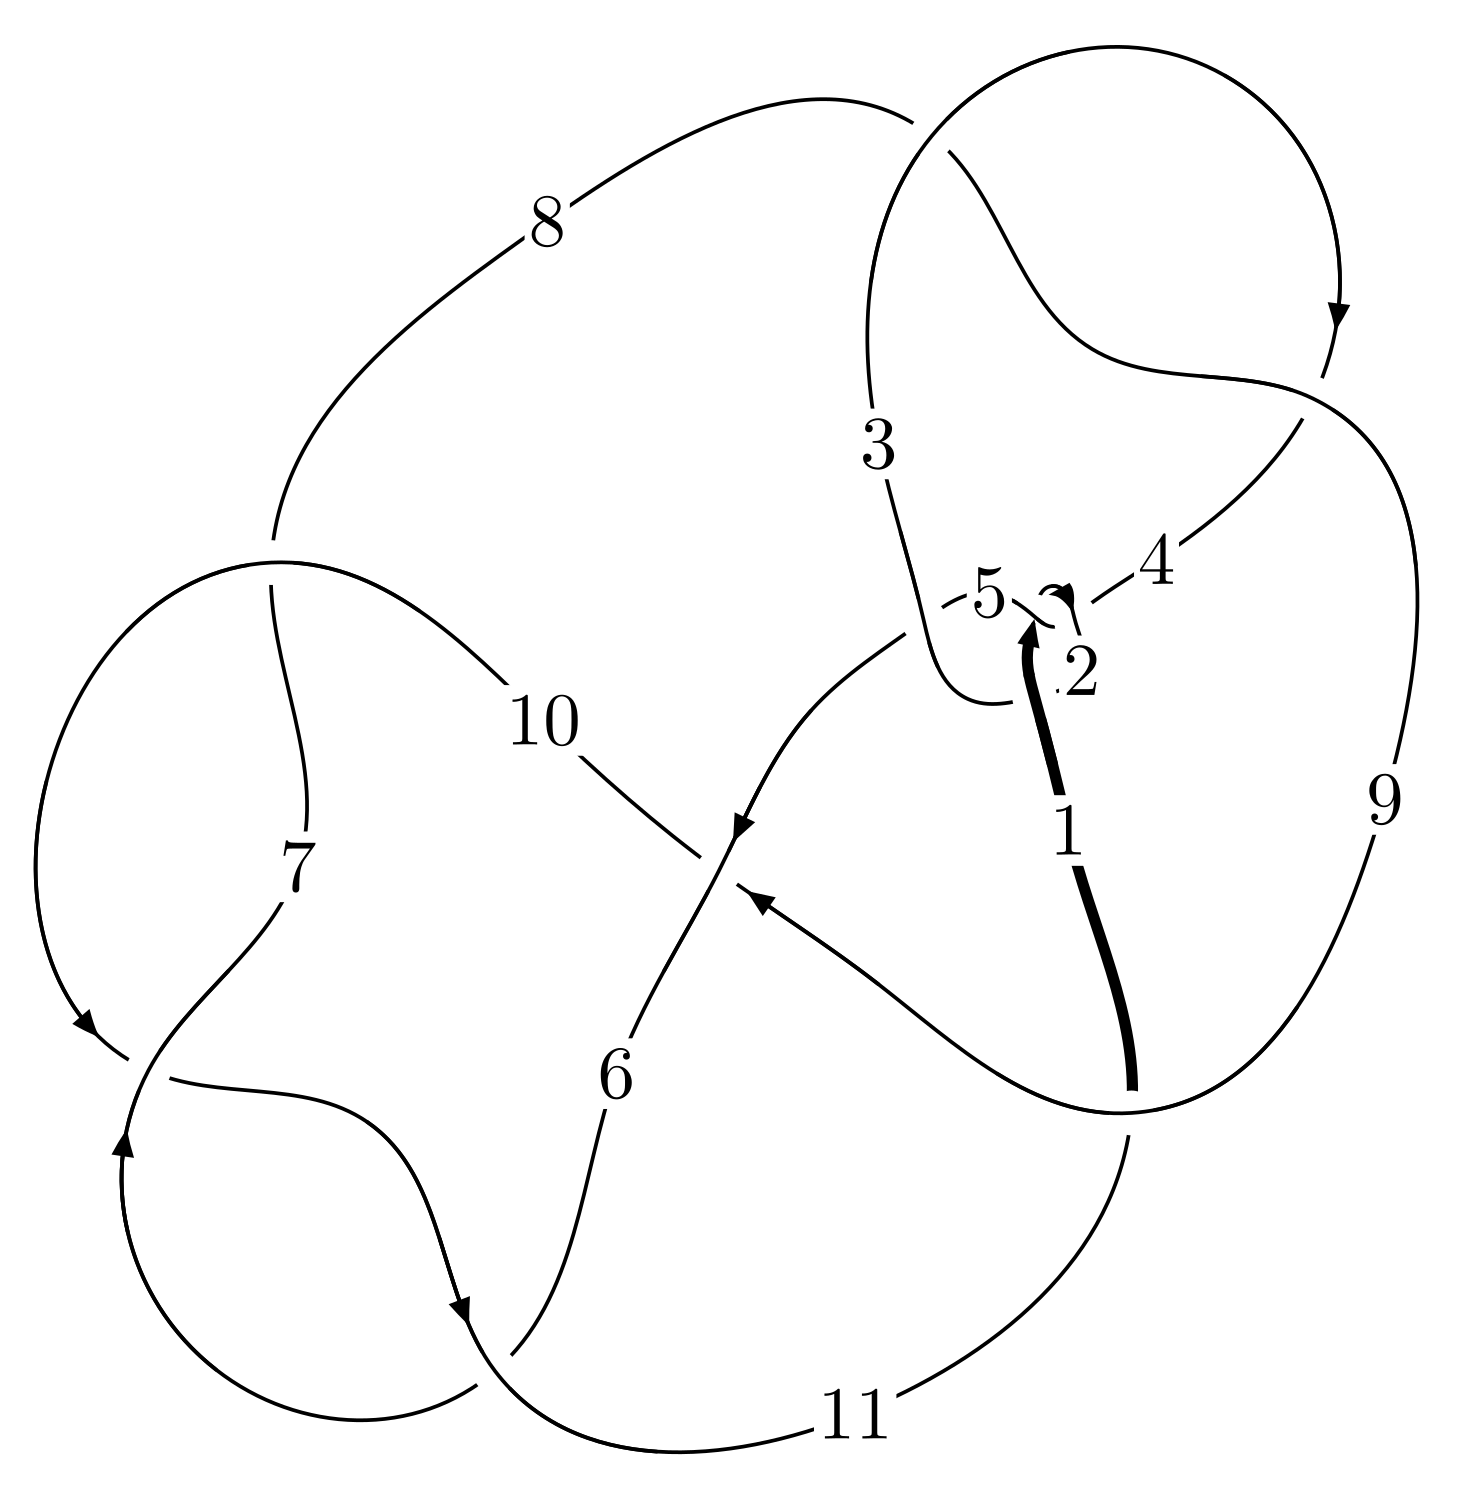
\includegraphics[width=112pt]{../../../GIT/diagram.site/Diagrams/png/633_11n_17.png}\\
\ \ \ A knot diagram\footnotemark}&
\allowdisplaybreaks
\textbf{Linearized knot diagam} \\
\cline{2-2}
 &
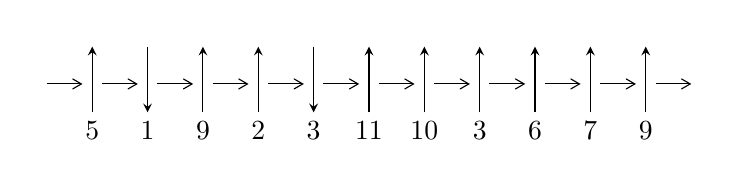
\begin{tikzpicture}[x=20pt, y=17pt]
	% nodes
	\node (C0) at (0, 0) {};
	\node (C1) at (1, 0) {};
	\node (C1U) at (1, +1) {};
	\node (C1D) at (1, -1) {5};

	\node (C2) at (2, 0) {};
	\node (C2U) at (2, +1) {};
	\node (C2D) at (2, -1) {1};

	\node (C3) at (3, 0) {};
	\node (C3U) at (3, +1) {};
	\node (C3D) at (3, -1) {9};

	\node (C4) at (4, 0) {};
	\node (C4U) at (4, +1) {};
	\node (C4D) at (4, -1) {2};

	\node (C5) at (5, 0) {};
	\node (C5U) at (5, +1) {};
	\node (C5D) at (5, -1) {3};

	\node (C6) at (6, 0) {};
	\node (C6U) at (6, +1) {};
	\node (C6D) at (6, -1) {11};

	\node (C7) at (7, 0) {};
	\node (C7U) at (7, +1) {};
	\node (C7D) at (7, -1) {10};

	\node (C8) at (8, 0) {};
	\node (C8U) at (8, +1) {};
	\node (C8D) at (8, -1) {3};

	\node (C9) at (9, 0) {};
	\node (C9U) at (9, +1) {};
	\node (C9D) at (9, -1) {6};

	\node (C10) at (10, 0) {};
	\node (C10U) at (10, +1) {};
	\node (C10D) at (10, -1) {7};

	\node (C11) at (11, 0) {};
	\node (C11U) at (11, +1) {};
	\node (C11D) at (11, -1) {9};
	\node (C12) at (12, 0) {};

	% arrows
	\draw[->,>={angle 60}]
	(C0) edge (C1) (C1) edge (C2) (C2) edge (C3) (C3) edge (C4) (C4) edge (C5) (C5) edge (C6) (C6) edge (C7) (C7) edge (C8) (C8) edge (C9) (C9) edge (C10) (C10) edge (C11) (C11) edge (C12) ;	\draw[->,>=stealth]
	(C1D) edge (C1U) (C2U) edge (C2D) (C3D) edge (C3U) (C4D) edge (C4U) (C5U) edge (C5D) (C6D) edge (C6U) (C7D) edge (C7U) (C8D) edge (C8U) (C9D) edge (C9U) (C10D) edge (C10U) (C11D) edge (C11U) ;
	\end{tikzpicture} \\
\hhline{~~} \\& 
\textbf{Solving Sequence} \\ \cline{2-2} 
 &
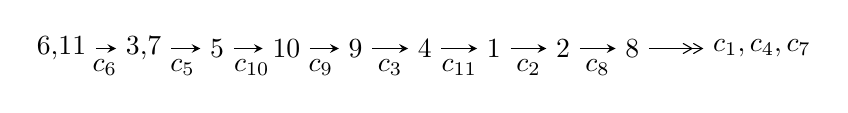
\begin{tikzpicture}[x=25pt, y=7pt]
	% node
	\node (A0) at (-1/8, 0) {6,11};
	\node (A1) at (17/16, 0) {3,7};
	\node (A2) at (17/8, 0) {5};
	\node (A3) at (25/8, 0) {10};
	\node (A4) at (33/8, 0) {9};
	\node (A5) at (41/8, 0) {4};
	\node (A6) at (49/8, 0) {1};
	\node (A7) at (57/8, 0) {2};
	\node (A8) at (65/8, 0) {8};
	\node (C1) at (1/2, -1) {$c_{6}$};
	\node (C2) at (13/8, -1) {$c_{5}$};
	\node (C3) at (21/8, -1) {$c_{10}$};
	\node (C4) at (29/8, -1) {$c_{9}$};
	\node (C5) at (37/8, -1) {$c_{3}$};
	\node (C6) at (45/8, -1) {$c_{11}$};
	\node (C7) at (53/8, -1) {$c_{2}$};
	\node (C8) at (61/8, -1) {$c_{8}$};
	\node (A9) at (10, 0) {$c_{1},c_{4},c_{7}$};

	% edge
	\draw[->,>=stealth]	
	(A0) edge (A1) (A1) edge (A2) (A2) edge (A3) (A3) edge (A4) (A4) edge (A5) (A5) edge (A6) (A6) edge (A7) (A7) edge (A8) ;
	\draw[->>,>={angle 60}]	
	(A8) edge (A9);
\end{tikzpicture} \\ 

\end{tabular} \\

\footnotetext{
The image of knot diagram is generated by the software ``\textbf{Draw programme}" developed by Andrew Bartholomew(\url{http://www.layer8.co.uk/maths/draw/index.htm\#Running-draw}), where we modified some parts for our purpose(\url{https://github.com/CATsTAILs/LinksPainter}).
}\phantom \\ \newline 
\centering \textbf{Ideals for irreducible components\footnotemark of $X_{\text{par}}$} 
 
\begin{align*}
I^u_{1}&=\langle 
u^{28}-2 u^{27}+\cdots+2 b-3,\;-3 u^{28}+8 u^{27}+\cdots+2 a+12,\;u^{29}-3 u^{28}+\cdots-4 u+1\rangle \\
I^u_{2}&=\langle 
- a u+b,\;- u^2 a+a^2- a u+2 u^2-2 a+u+3,\;u^3+u^2+2 u+1\rangle \\
\\
\end{align*}
\raggedright * 2 irreducible components of $\dim_{\mathbb{C}}=0$, with total 35 representations.\\
\footnotetext{All coefficients of polynomials are rational numbers. But the coefficients are sometimes approximated in decimal forms when there is not enough margin.}
\newpage
\renewcommand{\arraystretch}{1}
\centering \section*{I. $I^u_{1}= \langle u^{28}-2 u^{27}+\cdots+2 b-3,\;-3 u^{28}+8 u^{27}+\cdots+2 a+12,\;u^{29}-3 u^{28}+\cdots-4 u+1 \rangle$}
\flushleft \textbf{(i) Arc colorings}\\
\begin{tabular}{m{7pt} m{180pt} m{7pt} m{180pt} }
\flushright $a_{6}=$&$\begin{pmatrix}1\\0\end{pmatrix}$ \\
\flushright $a_{11}=$&$\begin{pmatrix}0\\u\end{pmatrix}$ \\
\flushright $a_{3}=$&$\begin{pmatrix}\frac{3}{2} u^{28}-4 u^{27}+\cdots+8 u-6\\-\frac{1}{2} u^{28}+u^{27}+\cdots-8 u^2+\frac{3}{2}\end{pmatrix}$ \\
\flushright $a_{7}=$&$\begin{pmatrix}1\\- u^2\end{pmatrix}$ \\
\flushright $a_{5}=$&$\begin{pmatrix}-\frac{1}{2} u^{28}+u^{27}+\cdots-6 u+1\\\frac{1}{2} u^{28}- u^{27}+\cdots+2 u-\frac{1}{2}\end{pmatrix}$ \\
\flushright $a_{10}=$&$\begin{pmatrix}- u\\u^3+u\end{pmatrix}$ \\
\flushright $a_{9}=$&$\begin{pmatrix}- u^3-2 u\\u^3+u\end{pmatrix}$ \\
\flushright $a_{4}=$&$\begin{pmatrix}\frac{1}{2} u^{28}-2 u^{27}+\cdots+6 u-6\\\frac{1}{2} u^{28}- u^{27}+\cdots+u+\frac{3}{2}\end{pmatrix}$ \\
\flushright $a_{1}=$&$\begin{pmatrix}u^7+4 u^5+4 u^3\\- u^7-3 u^5-2 u^3+u\end{pmatrix}$ \\
\flushright $a_{2}=$&$\begin{pmatrix}3 u^{28}-7 u^{27}+\cdots+11 u-\frac{13}{2}\\-\frac{5}{2} u^{28}+7 u^{27}+\cdots-6 u+\frac{7}{2}\end{pmatrix}$ \\
\flushright $a_{8}=$&$\begin{pmatrix}u^2+1\\- u^4-2 u^2\end{pmatrix}$\\ \flushright $a_{8}=$&$\begin{pmatrix}u^2+1\\- u^4-2 u^2\end{pmatrix}$\\&\end{tabular}
\flushleft \textbf{(ii) Obstruction class $= -1$}\\~\\
\flushleft \textbf{(iii) Cusp Shapes $= -2 u^{28}+\frac{7}{2} u^{27}+\cdots-\frac{33}{2} u+\frac{19}{2}$}\\~\\
\newpage\renewcommand{\arraystretch}{1}
\flushleft \textbf{(iv) u-Polynomials at the component}\newline \\
\begin{tabular}{m{50pt}|m{274pt}}
Crossings & \hspace{64pt}u-Polynomials at each crossing \\
\hline $$\begin{aligned}c_{1},c_{4}\end{aligned}$$&$\begin{aligned}
&u^{29}+4 u^{28}+\cdots+u-1
\end{aligned}$\\
\hline $$\begin{aligned}c_{2}\end{aligned}$$&$\begin{aligned}
&u^{29}+18 u^{28}+\cdots+9 u-1
\end{aligned}$\\
\hline $$\begin{aligned}c_{3},c_{8}\end{aligned}$$&$\begin{aligned}
&u^{29}- u^{28}+\cdots-32 u-64
\end{aligned}$\\
\hline $$\begin{aligned}c_{5}\end{aligned}$$&$\begin{aligned}
&u^{29}-4 u^{28}+\cdots+7 u-1
\end{aligned}$\\
\hline $$\begin{aligned}c_{6},c_{7},c_{10}\end{aligned}$$&$\begin{aligned}
&u^{29}+3 u^{28}+\cdots-4 u-1
\end{aligned}$\\
\hline $$\begin{aligned}c_{9}\end{aligned}$$&$\begin{aligned}
&u^{29}-3 u^{28}+\cdots-244 u-73
\end{aligned}$\\
\hline $$\begin{aligned}c_{11}\end{aligned}$$&$\begin{aligned}
&u^{29}+3 u^{28}+\cdots+8 u^2-1
\end{aligned}$\\
\hline
\end{tabular}\\~\\
\newpage\renewcommand{\arraystretch}{1}
\flushleft \textbf{(v) Riley Polynomials at the component}\newline \\
\begin{tabular}{m{50pt}|m{274pt}}
Crossings & \hspace{64pt}Riley Polynomials at each crossing \\
\hline $$\begin{aligned}c_{1},c_{4}\end{aligned}$$&$\begin{aligned}
&y^{29}+18 y^{28}+\cdots+9 y-1
\end{aligned}$\\
\hline $$\begin{aligned}c_{2}\end{aligned}$$&$\begin{aligned}
&y^{29}-10 y^{28}+\cdots+425 y-1
\end{aligned}$\\
\hline $$\begin{aligned}c_{3},c_{8}\end{aligned}$$&$\begin{aligned}
&y^{29}+35 y^{28}+\cdots-31744 y-4096
\end{aligned}$\\
\hline $$\begin{aligned}c_{5}\end{aligned}$$&$\begin{aligned}
&y^{29}-38 y^{28}+\cdots+9 y-1
\end{aligned}$\\
\hline $$\begin{aligned}c_{6},c_{7},c_{10}\end{aligned}$$&$\begin{aligned}
&y^{29}+29 y^{28}+\cdots+16 y-1
\end{aligned}$\\
\hline $$\begin{aligned}c_{9}\end{aligned}$$&$\begin{aligned}
&y^{29}+17 y^{28}+\cdots+23912 y-5329
\end{aligned}$\\
\hline $$\begin{aligned}c_{11}\end{aligned}$$&$\begin{aligned}
&y^{29}+37 y^{28}+\cdots+16 y-1
\end{aligned}$\\
\hline
\end{tabular}\\~\\
\newpage\flushleft \textbf{(vi) Complex Volumes and Cusp Shapes}
$$\begin{array}{c|c|c}  
\text{Solutions to }I^u_{1}& \I (\text{vol} + \sqrt{-1}CS) & \text{Cusp shape}\\
 \hline 
\begin{aligned}
u &= \phantom{-}0.691423 + 0.598710 I \\
a &= \phantom{-}1.37569 - 1.31340 I \\
b &= -1.73753 + 0.08448 I\end{aligned}
 & -8.85458 - 2.60938 I & \phantom{-}2.88623 + 0.30936 I \\ \hline\begin{aligned}
u &= \phantom{-}0.691423 - 0.598710 I \\
a &= \phantom{-}1.37569 + 1.31340 I \\
b &= -1.73753 - 0.08448 I\end{aligned}
 & -8.85458 + 2.60938 I & \phantom{-}2.88623 - 0.30936 I \\ \hline\begin{aligned}
u &= \phantom{-}0.770996 + 0.462752 I \\
a &= \phantom{-}1.67161 - 1.26096 I \\
b &= -1.87232 + 0.19865 I\end{aligned}
 & -8.40111 + 7.50786 I & \phantom{-}3.89559 - 5.68378 I \\ \hline\begin{aligned}
u &= \phantom{-}0.770996 - 0.462752 I \\
a &= \phantom{-}1.67161 + 1.26096 I \\
b &= -1.87232 - 0.19865 I\end{aligned}
 & -8.40111 - 7.50786 I & \phantom{-}3.89559 + 5.68378 I \\ \hline\begin{aligned}
u &= \phantom{-}0.690364 + 0.493803 I \\
a &= -1.54905 + 1.40959 I \\
b &= \phantom{-}1.76547 - 0.20820 I\end{aligned}
 & -4.66644 + 2.28896 I & \phantom{-}6.38324 - 2.89322 I \\ \hline\begin{aligned}
u &= \phantom{-}0.690364 - 0.493803 I \\
a &= -1.54905 - 1.40959 I \\
b &= \phantom{-}1.76547 + 0.20820 I\end{aligned}
 & -4.66644 - 2.28896 I & \phantom{-}6.38324 + 2.89322 I \\ \hline\begin{aligned}
u &= -0.171803 + 1.253430 I \\
a &= -0.337041 + 0.105101 I \\
b &= \phantom{-}0.073833 + 0.440514 I\end{aligned}
 & -2.92626 - 2.06352 I & \phantom{-}3.82434 + 4.59366 I \\ \hline\begin{aligned}
u &= -0.171803 - 1.253430 I \\
a &= -0.337041 - 0.105101 I \\
b &= \phantom{-}0.073833 - 0.440514 I\end{aligned}
 & -2.92626 + 2.06352 I & \phantom{-}3.82434 - 4.59366 I \\ \hline\begin{aligned}
u &= -0.674782 + 0.131684 I \\
a &= -0.108599 - 0.371194 I \\
b &= -0.122161 - 0.236174 I\end{aligned}
 & \phantom{-}0.280276 - 0.752914 I & \phantom{-}5.99242 + 0.52273 I \\ \hline\begin{aligned}
u &= -0.674782 - 0.131684 I \\
a &= -0.108599 + 0.371194 I \\
b &= -0.122161 + 0.236174 I\end{aligned}
 & \phantom{-}0.280276 + 0.752914 I & \phantom{-}5.99242 - 0.52273 I\\
 \hline 
 \end{array}$$\newpage$$\begin{array}{c|c|c}  
\text{Solutions to }I^u_{1}& \I (\text{vol} + \sqrt{-1}CS) & \text{Cusp shape}\\
 \hline 
\begin{aligned}
u &= -0.019678 + 1.322720 I \\
a &= -0.737573 - 0.279772 I \\
b &= -0.384574 + 0.970095 I\end{aligned}
 & -3.02767 - 1.44830 I & \phantom{-}4.95474 + 3.01169 I \\ \hline\begin{aligned}
u &= -0.019678 - 1.322720 I \\
a &= -0.737573 + 0.279772 I \\
b &= -0.384574 - 0.970095 I\end{aligned}
 & -3.02767 + 1.44830 I & \phantom{-}4.95474 - 3.01169 I \\ \hline\begin{aligned}
u &= -0.297090 + 1.319120 I \\
a &= \phantom{-}0.044330 - 0.313521 I \\
b &= -0.400401 - 0.151621 I\end{aligned}
 & -4.26542 - 4.32252 I & -0.05495 + 2.76648 I \\ \hline\begin{aligned}
u &= -0.297090 - 1.319120 I \\
a &= \phantom{-}0.044330 + 0.313521 I \\
b &= -0.400401 + 0.151621 I\end{aligned}
 & -4.26542 + 4.32252 I & -0.05495 - 2.76648 I \\ \hline\begin{aligned}
u &= \phantom{-}0.070374 + 1.382890 I \\
a &= \phantom{-}0.882690 + 0.761515 I \\
b &= \phantom{-}0.99097 - 1.27426 I\end{aligned}
 & -4.31077 + 3.55507 I & \phantom{-}1.62564 - 2.30473 I \\ \hline\begin{aligned}
u &= \phantom{-}0.070374 - 1.382890 I \\
a &= \phantom{-}0.882690 - 0.761515 I \\
b &= \phantom{-}0.99097 + 1.27426 I\end{aligned}
 & -4.31077 - 3.55507 I & \phantom{-}1.62564 + 2.30473 I \\ \hline\begin{aligned}
u &= -0.300475 + 0.478492 I \\
a &= \phantom{-}0.156143 + 0.882607 I \\
b &= \phantom{-}0.469237 + 0.190488 I\end{aligned}
 & -1.43996 - 2.11719 I & \phantom{-}2.79129 + 5.41296 I \\ \hline\begin{aligned}
u &= -0.300475 - 0.478492 I \\
a &= \phantom{-}0.156143 - 0.882607 I \\
b &= \phantom{-}0.469237 - 0.190488 I\end{aligned}
 & -1.43996 + 2.11719 I & \phantom{-}2.79129 - 5.41296 I \\ \hline\begin{aligned}
u &= -0.11472 + 1.46953 I \\
a &= \phantom{-}0.292500 + 0.496633 I \\
b &= \phantom{-}0.763375 - 0.372865 I\end{aligned}
 & -7.73410 - 3.73497 I & \phantom{-0.000000 -}0. + 3.25156 I \\ \hline\begin{aligned}
u &= -0.11472 - 1.46953 I \\
a &= \phantom{-}0.292500 - 0.496633 I \\
b &= \phantom{-}0.763375 + 0.372865 I\end{aligned}
 & -7.73410 + 3.73497 I & \phantom{-0.000000 } 0. - 3.25156 I\\
 \hline 
 \end{array}$$\newpage$$\begin{array}{c|c|c}  
\text{Solutions to }I^u_{1}& \I (\text{vol} + \sqrt{-1}CS) & \text{Cusp shape}\\
 \hline 
\begin{aligned}
u &= \phantom{-}0.24380 + 1.50275 I \\
a &= \phantom{-}0.103696 + 1.362120 I \\
b &= \phantom{-}2.02164 - 0.48792 I\end{aligned}
 & -11.15070 + 5.70562 I & \phantom{-}3.18778 - 2.80294 I \\ \hline\begin{aligned}
u &= \phantom{-}0.24380 - 1.50275 I \\
a &= \phantom{-}0.103696 - 1.362120 I \\
b &= \phantom{-}2.02164 + 0.48792 I\end{aligned}
 & -11.15070 - 5.70562 I & \phantom{-}3.18778 + 2.80294 I \\ \hline\begin{aligned}
u &= \phantom{-}0.28209 + 1.50525 I \\
a &= \phantom{-}0.024600 - 1.383480 I \\
b &= -2.08942 + 0.35324 I\end{aligned}
 & -14.7787 + 11.3588 I & \phantom{-}0.97389 - 5.82372 I \\ \hline\begin{aligned}
u &= \phantom{-}0.28209 - 1.50525 I \\
a &= \phantom{-}0.024600 + 1.383480 I \\
b &= -2.08942 - 0.35324 I\end{aligned}
 & -14.7787 - 11.3588 I & \phantom{-}0.97389 + 5.82372 I \\ \hline\begin{aligned}
u &= \phantom{-}0.21267 + 1.54249 I \\
a &= -0.131402 - 1.205960 I \\
b &= -1.83224 + 0.45916 I\end{aligned}
 & -15.9085 + 0.6657 I & \phantom{-0.000000 } 0 \\ \hline\begin{aligned}
u &= \phantom{-}0.21267 - 1.54249 I \\
a &= -0.131402 + 1.205960 I \\
b &= -1.83224 - 0.45916 I\end{aligned}
 & -15.9085 - 0.6657 I & \phantom{-0.000000 } 0 \\ \hline\begin{aligned}
u &= -0.417634\phantom{ +0.000000I} \\
a &= -0.553347\phantom{ +0.000000I} \\
b &= -0.231097\phantom{ +0.000000I}\end{aligned}
 & \phantom{-}0.741502\phantom{ +0.000000I} & \phantom{-}13.5070\phantom{ +0.000000I} \\ \hline\begin{aligned}
u &= \phantom{-}0.325642 + 0.098864 I \\
a &= -0.41093 + 3.39717 I \\
b &= \phantom{-}0.469675 - 1.065640 I\end{aligned}
 & \phantom{-}0.45415 + 2.26174 I & \phantom{-}0.65884 - 5.12612 I \\ \hline\begin{aligned}
u &= \phantom{-}0.325642 - 0.098864 I \\
a &= -0.41093 - 3.39717 I \\
b &= \phantom{-}0.469675 + 1.065640 I\end{aligned}
 & \phantom{-}0.45415 - 2.26174 I & \phantom{-}0.65884 + 5.12612 I\\
 \hline 
 \end{array}$$\newpage\newpage\renewcommand{\arraystretch}{1}
\centering \section*{II. $I^u_{2}= \langle - a u+b,\;- u^2 a+a^2- a u+2 u^2-2 a+u+3,\;u^3+u^2+2 u+1 \rangle$}
\flushleft \textbf{(i) Arc colorings}\\
\begin{tabular}{m{7pt} m{180pt} m{7pt} m{180pt} }
\flushright $a_{6}=$&$\begin{pmatrix}1\\0\end{pmatrix}$ \\
\flushright $a_{11}=$&$\begin{pmatrix}0\\u\end{pmatrix}$ \\
\flushright $a_{3}=$&$\begin{pmatrix}a\\a u\end{pmatrix}$ \\
\flushright $a_{7}=$&$\begin{pmatrix}1\\- u^2\end{pmatrix}$ \\
\flushright $a_{5}=$&$\begin{pmatrix}- u^2+a- u-1\\a u+1\end{pmatrix}$ \\
\flushright $a_{10}=$&$\begin{pmatrix}- u\\- u^2- u-1\end{pmatrix}$ \\
\flushright $a_{9}=$&$\begin{pmatrix}u^2+1\\- u^2- u-1\end{pmatrix}$ \\
\flushright $a_{4}=$&$\begin{pmatrix}a\\a u\end{pmatrix}$ \\
\flushright $a_{1}=$&$\begin{pmatrix}-1\\0\end{pmatrix}$ \\
\flushright $a_{2}=$&$\begin{pmatrix}a u+a\\a u\end{pmatrix}$ \\
\flushright $a_{8}=$&$\begin{pmatrix}u^2+1\\- u^2- u-1\end{pmatrix}$\\ \flushright $a_{8}=$&$\begin{pmatrix}u^2+1\\- u^2- u-1\end{pmatrix}$\\&\end{tabular}
\flushleft \textbf{(ii) Obstruction class $= 1$}\\~\\
\flushleft \textbf{(iii) Cusp Shapes $= u^2 a-4 a u+5 u^2- a+5 u+12$}\\~\\
\newpage\renewcommand{\arraystretch}{1}
\flushleft \textbf{(iv) u-Polynomials at the component}\newline \\
\begin{tabular}{m{50pt}|m{274pt}}
Crossings & \hspace{64pt}u-Polynomials at each crossing \\
\hline $$\begin{aligned}c_{1},c_{2},c_{5}\end{aligned}$$&$\begin{aligned}
&(u^2+u+1)^3
\end{aligned}$\\
\hline $$\begin{aligned}c_{3},c_{8}\end{aligned}$$&$\begin{aligned}
&u^6
\end{aligned}$\\
\hline $$\begin{aligned}c_{4}\end{aligned}$$&$\begin{aligned}
&(u^2- u+1)^3
\end{aligned}$\\
\hline $$\begin{aligned}c_{6},c_{7}\end{aligned}$$&$\begin{aligned}
&(u^3+u^2+2 u+1)^2
\end{aligned}$\\
\hline $$\begin{aligned}c_{9},c_{11}\end{aligned}$$&$\begin{aligned}
&(u^3+u^2-1)^2
\end{aligned}$\\
\hline $$\begin{aligned}c_{10}\end{aligned}$$&$\begin{aligned}
&(u^3- u^2+2 u-1)^2
\end{aligned}$\\
\hline
\end{tabular}\\~\\
\newpage\renewcommand{\arraystretch}{1}
\flushleft \textbf{(v) Riley Polynomials at the component}\newline \\
\begin{tabular}{m{50pt}|m{274pt}}
Crossings & \hspace{64pt}Riley Polynomials at each crossing \\
\hline $$\begin{aligned}c_{1},c_{2},c_{4}\\c_{5}\end{aligned}$$&$\begin{aligned}
&(y^2+y+1)^3
\end{aligned}$\\
\hline $$\begin{aligned}c_{3},c_{8}\end{aligned}$$&$\begin{aligned}
&y^6
\end{aligned}$\\
\hline $$\begin{aligned}c_{6},c_{7},c_{10}\end{aligned}$$&$\begin{aligned}
&(y^3+3 y^2+2 y-1)^2
\end{aligned}$\\
\hline $$\begin{aligned}c_{9},c_{11}\end{aligned}$$&$\begin{aligned}
&(y^3- y^2+2 y-1)^2
\end{aligned}$\\
\hline
\end{tabular}\\~\\
\newpage\flushleft \textbf{(vi) Complex Volumes and Cusp Shapes}
$$\begin{array}{c|c|c}  
\text{Solutions to }I^u_{2}& \I (\text{vol} + \sqrt{-1}CS) & \text{Cusp shape}\\
 \hline 
\begin{aligned}
u &= -0.215080 + 1.307140 I \\
a &= \phantom{-}0.706350 + 0.266290 I \\
b &= -0.500000 + 0.866025 I\end{aligned}
 & -3.02413 - 4.85801 I & \phantom{-}6.43615 + 6.24253 I \\ \hline\begin{aligned}
u &= -0.215080 + 1.307140 I \\
a &= -0.583789 + 0.478572 I \\
b &= -0.500000 - 0.866025 I\end{aligned}
 & -3.02413 - 0.79824 I & \phantom{-}2.88198 - 0.84592 I \\ \hline\begin{aligned}
u &= -0.215080 - 1.307140 I \\
a &= \phantom{-}0.706350 - 0.266290 I \\
b &= -0.500000 - 0.866025 I\end{aligned}
 & -3.02413 + 4.85801 I & \phantom{-}6.43615 - 6.24253 I \\ \hline\begin{aligned}
u &= -0.215080 - 1.307140 I \\
a &= -0.583789 - 0.478572 I \\
b &= -0.500000 + 0.866025 I\end{aligned}
 & -3.02413 + 0.79824 I & \phantom{-}2.88198 + 0.84592 I \\ \hline\begin{aligned}
u &= -0.569840\phantom{ +0.000000I} \\
a &= \phantom{-}0.87744 + 1.51977 I \\
b &= -0.500000 - 0.866025 I\end{aligned}
 & \phantom{-}1.11345 - 2.02988 I & \phantom{-}12.18187 + 2.43783 I \\ \hline\begin{aligned}
u &= -0.569840\phantom{ +0.000000I} \\
a &= \phantom{-}0.87744 - 1.51977 I \\
b &= -0.500000 + 0.866025 I\end{aligned}
 & \phantom{-}1.11345 + 2.02988 I & \phantom{-}12.18187 - 2.43783 I\\
 \hline 
 \end{array}$$\newpage
\newpage\renewcommand{\arraystretch}{1}
\centering \section*{ III. u-Polynomials}
\begin{tabular}{m{50pt}|m{274pt}}
Crossings & \hspace{64pt}u-Polynomials at each crossing \\
\hline $$\begin{aligned}c_{1}\end{aligned}$$&$\begin{aligned}
&((u^2+u+1)^3)(u^{29}+4 u^{28}+\cdots+u-1)
\end{aligned}$\\
\hline $$\begin{aligned}c_{2}\end{aligned}$$&$\begin{aligned}
&((u^2+u+1)^3)(u^{29}+18 u^{28}+\cdots+9 u-1)
\end{aligned}$\\
\hline $$\begin{aligned}c_{3},c_{8}\end{aligned}$$&$\begin{aligned}
&u^6(u^{29}- u^{28}+\cdots-32 u-64)
\end{aligned}$\\
\hline $$\begin{aligned}c_{4}\end{aligned}$$&$\begin{aligned}
&((u^2- u+1)^3)(u^{29}+4 u^{28}+\cdots+u-1)
\end{aligned}$\\
\hline $$\begin{aligned}c_{5}\end{aligned}$$&$\begin{aligned}
&((u^2+u+1)^3)(u^{29}-4 u^{28}+\cdots+7 u-1)
\end{aligned}$\\
\hline $$\begin{aligned}c_{6},c_{7}\end{aligned}$$&$\begin{aligned}
&((u^3+u^2+2 u+1)^2)(u^{29}+3 u^{28}+\cdots-4 u-1)
\end{aligned}$\\
\hline $$\begin{aligned}c_{9}\end{aligned}$$&$\begin{aligned}
&((u^3+u^2-1)^2)(u^{29}-3 u^{28}+\cdots-244 u-73)
\end{aligned}$\\
\hline $$\begin{aligned}c_{10}\end{aligned}$$&$\begin{aligned}
&((u^3- u^2+2 u-1)^2)(u^{29}+3 u^{28}+\cdots-4 u-1)
\end{aligned}$\\
\hline $$\begin{aligned}c_{11}\end{aligned}$$&$\begin{aligned}
&((u^3+u^2-1)^2)(u^{29}+3 u^{28}+\cdots+8 u^2-1)
\end{aligned}$\\
\hline
\end{tabular}\newpage\renewcommand{\arraystretch}{1}
\centering \section*{ IV. Riley Polynomials}
\begin{tabular}{m{50pt}|m{274pt}}
Crossings & \hspace{64pt}Riley Polynomials at each crossing \\
\hline $$\begin{aligned}c_{1},c_{4}\end{aligned}$$&$\begin{aligned}
&((y^2+y+1)^3)(y^{29}+18 y^{28}+\cdots+9 y-1)
\end{aligned}$\\
\hline $$\begin{aligned}c_{2}\end{aligned}$$&$\begin{aligned}
&((y^2+y+1)^3)(y^{29}-10 y^{28}+\cdots+425 y-1)
\end{aligned}$\\
\hline $$\begin{aligned}c_{3},c_{8}\end{aligned}$$&$\begin{aligned}
&y^6(y^{29}+35 y^{28}+\cdots-31744 y-4096)
\end{aligned}$\\
\hline $$\begin{aligned}c_{5}\end{aligned}$$&$\begin{aligned}
&((y^2+y+1)^3)(y^{29}-38 y^{28}+\cdots+9 y-1)
\end{aligned}$\\
\hline $$\begin{aligned}c_{6},c_{7},c_{10}\end{aligned}$$&$\begin{aligned}
&((y^3+3 y^2+2 y-1)^2)(y^{29}+29 y^{28}+\cdots+16 y-1)
\end{aligned}$\\
\hline $$\begin{aligned}c_{9}\end{aligned}$$&$\begin{aligned}
&((y^3- y^2+2 y-1)^2)(y^{29}+17 y^{28}+\cdots+23912 y-5329)
\end{aligned}$\\
\hline $$\begin{aligned}c_{11}\end{aligned}$$&$\begin{aligned}
&((y^3- y^2+2 y-1)^2)(y^{29}+37 y^{28}+\cdots+16 y-1)
\end{aligned}$\\
\hline
\end{tabular}
\vskip 2pc
\end{document}